%\documentclass[12pt,ascmac]{jreport}
\documentclass[12pt]{jreport}
\usepackage{./sty/eclepsf}
\usepackage{tascmac}
\usepackage{tabularx}
\usepackage[longnamesfirst]{natbib}
\usepackage[dvipdfmx]{graphics}
\usepackage[dvipdfmx]{graphicx}
\usepackage[dvipdfmx]{color}
\usepackage{subfigure}
\usepackage{alltt}
\usepackage{./sty/ncodeline}
%\usepackage[dvipdfmx, colorlinks, breaklinks,%
\usepackage[dvipdfmx, breaklinks,%
bookmarks=true, bookmarksnumbered=true,%
bookmarkstype=toc, bookmarksopen=true,bookmarksopenlevel=3,%
pdftitle={Design and Implementation of Swift Parser Written in Swift for Bootstrapping},%
%%pdfsubject={},%
pdfauthor={Atsuki Demizu},%
pdfkeywords={1.Bootstrap a Compiler, 2.Parser, 3.Implementation of Parser, 4.Swift Programming Language}%
]{hyperref}
\usepackage{bookmark}

\AtBeginDvi{\special{pdf:tounicode EUC-UCS2}}

\usepackage{fancyhdr}

\usepackage{./sty/doxygenorig}

\usepackage{indentfirst}
\usepackage{url}
\usepackage{listings,./sty/jlisting}

\lstset{%
 language={C++},
 %backgroundcolor={\color[gray]{.85}},%
 basicstyle={\small\ttfamily},%
 identifierstyle={\small},%
 commentstyle={\small\itshape},%
 keywordstyle={\small\bfseries},%
 ndkeywordstyle={\small\ttfamily},%
 stringstyle={\small\ttfamily},
 frame={tb},
 framesep=1zw,
 breaklines=true,
 numbers=left,%
 xrightmargin=0zw,%
 xleftmargin=1.5zw,%
 numberstyle={\scriptsize},%
 stepnumber=1,
 numbersep=1zw,%
 lineskip=-0.5ex%
}

\usepackage{amssymb}
%\usepackage{supertabular,multirow}

% A4  size: 297mm*210mm %1pt = 0.35mm
\setlength{\topmargin}{-3.4mm} % 10pt 25.4mm - 3.4mm = 22mm
\setlength{\oddsidemargin}{-0.4mm} % 25.4mm - 0.4mm = 25mm
\setlength{\evensidemargin}{-0.4mm} % 25.4mm - 0.4mm = 25mm
\setlength{\textheight}{231mm} % 660pt % original is 225.75mm 645pt
\setlength{\textwidth}{160mm} % 457pt

\renewcommand{\topfraction}{.99}
\renewcommand{\textfraction}{.0}
\renewcommand{\floatpagefraction}{.99}
\renewcommand{\bibname}{参考文献}

\pagestyle{fancy}  
%\rhead{\thepage}
%\rhead[]{\leftmark} 
\lhead[]{} 
%\lhead[\rightmark]{} 

\makeatletter
\def\chaptermark#1{\markboth {\ifnum \c@secnumdepth>\m@ne
\@chapapp\ \thechapter \@chappos\ \fi #1}{}}
\makeatother

\begin{document}

\pagenumbering{roman}

\begin{titlepage}
  \begin{center}
    \begin{large}
      卒業論文   2015年度(平成27年)\\
      \vspace{24pt}
      Self-host化によるSwiftコンパイラのソースコード可読性の向上
      \end{large}
  \end{center}
  \vspace{40em}
  \begin{flushright}
    \large 慶應義塾大学 環境情報学部\\
    出水 厚輝
  \end{flushright}
\end{titlepage}


\thispagestyle{empty}
卒業論文要旨 - 2015年度 (平成27年度)
\begin{center}
\begin{Large}
\begin{tabular}{|c|} \hline
Self-host化によるSwiftコンパイラのソースコード可読性の向上
\\ \hline
\end{tabular}
\end{Large}
\end{center}
%~ \bigskip ~ \\

オープンソースとなったソフトウェアにおいては、その開発に関わるプログラマの増加とそれに伴うプログラムの修正や機能追加の増加によって、そのソースコードの可読性が拡張やそれに対するレビューの容易さに影響し、プロジェクト自体の成否に大きく関わる場合がある。

2015年12月にオープンソースとなったApple社が中心となって開発しているプログラミング言語Swiftもそうした可能性の分岐点に立つソフトウェアの1つである。
現在Swiftコンパイラの可読性は既存コードのコーディングスタイルへの習慣的な追従とレビューの徹底によって保たれているが、この形だけでは新しいコードの増加やプロジェクトメンバーの交代などによってその可読性が保てなくなる可能性が高い。

一方で、Swiftでは行われていないものの、現在利用されている多くの高級な汎用プログラミング言語では、コンパイル対象となる言語自体でそのコンパイラを記述するSelf-host化がよく行われている。
Self-host化を行うことによるメリットはいくつかあるが、たびたびモチベーションとしてあげられるのは、その可読性における優位点である。
コンパイラを記述する言語とその対象言語が同じになれば開発者はより少ない知識でコンパイラのコードを読むことができる上、初期のコンパイラにおいては、それを記述している言語よりもそのコンパイル対象となっている言語のほうが必ず後発のものであるため、多くの場合により表現力が高く、可読性においてもより高い水準となるからである。

そこで本研究では、Swiftで記述されたSwiftコンパイラの構文解析器を実装し、現行のSwiftコンパイラの構文解析器とそのソースコードの行数を多面的に比較することでSelf-host化がSwiftコンパイラに与える影響についての検証を行った。
検証の結果として、本論文ではSwiftコンパイラのSelf-host化によってその可読性が向上する可能性が十分にあることを示している。
だだし、同時に行ったSelf-host化に伴うデメリットの考察により、Self-host化がコンパイラに対して与える他の影響を鑑みると、実際の適用に際してはより慎重にならなければいけないということもわかった。

~ \\
キーワード:\\
\underline{1. コンパイラ},
\underline{2. Self-host化},
\underline{3. プログラムの可読性},\\
\underline{4. プログラミング言語Swift}
\begin{flushright}
慶應義塾大学 環境情報学部\\
出水 厚輝
\end{flushright}

\clearpage

\thispagestyle{empty}
Abstract of Bachelor's Thesis - Academic Year 2015
\begin{center}
\begin{large}
\begin{tabular}{|p{0.97\linewidth}|}
    \hline
    Improvement of the Readability of Swift Compiler's Source Code by Self-hosting\\
    \hline
\end{tabular}
\end{large}
\end{center}

~ \\

When the software project changes into an open source, as both the number of joining developpers \& the extension/modification of program increase, the readability of software's source code becomes important factor for succeeding the project.

In December 2015, the Swift programming language project, which is leaded by Apple, made its souce code public and started to face with such a change.
In current process, the readability of Swift compiler is maintained just by the effort to habitually follow the coding style of existing codes and its strict review.
Therefore, when the new codes grows wider in the software, its readability should become out of control.

On the other hand, there is a technique called Self-hosting, which is adopted in many general-purpose high-level programming languages.
The Self-hosting is a technique writing the compiler in its targeting programming language.
Although there are multiple reasons to adopt the Self-hosting to the compile, the most attractive advantage is that developers can reduce their effort for understanding the software.
When the compiler is self-hosted, its developpers are not reqired to learn the other than the targeting language.
And furthermore, as the targeting language is newer than its compiler's description language in the early years, the Self-hosting has an effect to change the compiler's source code less complex with the new and expressive grammars of targeting language.

In this research, we implemented the new Swift compiler which is written by Swift and compare its parser with the parser of Apple's Swift compiler in order to verify the readability enhancement ability of Self-hosting.
As the result of this research, we colud confirm the positive effect of Self-hosting on the readability.
But at the same time, as the effect depends on some characteristic grammars of Swift, we are considering that some other languages whose compiler is written by other high-level language may not be benefited the effect.

~ \\
Keywords : \\
\underline{1. Compiler},
\underline{2. Self-hosting},
\underline{3. Readability of Program},\\
\underline{4. Swift Programming Language}
\begin{flushright}
Keio University, Faculty of Environment and Information Studies\\
Atsuki Demizu
\end{flushright}

\clearpage

\tableofcontents\thispagestyle{empty} %目次
\clearpage
\listoffigures\thispagestyle{empty} %図目次
\clearpage
\listoftables\thispagestyle{empty} %表目次
\clearpage
\pagenumbering{arabic}
\chapter{序論}
\label{introduction}

\section{背景}
\label{introduction:background}

2015年12月4日、Apple社が予てより同社の提供するCocoaおよびCocoa Touchフレームワークを用いたソフトウェアの開発用として提供していたプログラミング言語Swiftをオープンソース化し、Linuxを中心としたさまざまなプラットフォームにおけるソフトウェアを開発するための拡張を開始した。
これによりプログラミング言語SwiftはObjective-Cの担ってきたiOSやMac OS Xなどにおけるソフトウェアの開発だけでなく、C++やJavaなど他の汎用プログラミング言語が担ってきたソフトウェア開発においても、それらの代替となり得る可能性を持つこととなった。

Swiftはオブジェクト指向や全称型・存在型の導入、関数の第一級オブジェクト化、HindlyとMilnerによる型再構築アルゴリズムの採用など、現在多くのプログラマに使用されている他の汎用高級言語が持つ様々な特徴を持っているが、まだその特徴を採用するか否かがよく議論されていないものもある。
その内の1つがコンパイラをそのコンパイル対象の言語自体で開発するBootstrapプロセスの採用である。

表~\ref{table:bootstrapping-languages}はWeb検索エンジンにおけるクエリヒット数からプログラミング言語の知名度を格付けしたTIOBE Indexの2015年12月版において上げられている言語の内、汎用言語であるものだけを上位から20言語抽出し、それらの主要なコンパイラがその言語自体で記述されているかを示したものである。
この20言語の内だけでもBootstrapを行っているものが8言語あり、 その中に性能の問題からコンパイラ用の言語として採用されづらいインタプリタ型言語なども含まれていることを考慮すれば、かなりの言語がBootstrapされていることが分かる。
しかし、現在SwiftはC++を用いて開発されており、Bootstrapは行われていない。

現在Swiftにおいては未だ多くの機能が不足しており、他の問題を優先しているためにBootstrapについて大きく取り上げられてはいない。
また、開発者のメーリングリスト~\cite{dev-ml}では特にSwiftコンパイラのバックエンドとして採用されているLLVMのAPIがC++で提供されていることから、SwiftがC++と同様の役割を果たすにはもう少し時間が必要だという意見も上がっている。


しかし、~\ref{explain-bootstrap:merit}節で述べるようにBootstrapを行うことで得られる利益があることが他の言語の事例によって示されている以上、十分な議論なしに現状のSwiftにBootstrapが不要であると判断するのは早計であるといえる。

\begin{table}[tb]
    \begin{center}
        \caption{知名度の高いプログラミング言語のBootstrap状況}
        \begin{tabular}{|c|c|c|c|}
            \hline
            順位 & 言語名 & コンパイラ名 & Bootstrap状況 \\
            \hline
            1 & Java & javac & N (C, C++?) \\
            \hline
            1 & Java & OpenJDK & N (C++, Java) \\
            \hline
            2 & C & gcc & N (C++) \\
            \hline
            2 & C & clang & N (C++) \\
            \hline
            3 & C++ & gcc & Y \\
            \hline
            3 & C++ & clang & Y \\
            \hline
            3 & C++ & Microsoft Visual C++ & Y \\
            \hline
            4 & Python & cpython & N (C) \\
            \hline
            4 & Python & PyPy & Y \\
            \hline
            5 & C\# & Microsoft Visual C\# & N (C++) \\
            \hline
            5 & C\# & .NET Compiler Platform (Roslyn) & Y \\
            \hline
            6 & PHP & Zend Engine & N (C) \\
            \hline
            7 & Visual Basic .NET & Visual Studio & N (C++, C\#) \\
            \hline
            7 & Visual Basic .NET & .NET Compiler Platform (Roslyn) & Y \\
            \hline
            8 & JavaScript & SpiderMonkey & N (C, C++) \\
            \hline
            8 & JavaScript & V8 & N (C++, JavaScript) \\
            \hline
            9 & Perl & perl & N (C) \\
            \hline
            10 & Ruby & Ruby MRI & N (C) \\
            \hline
            12 & Visual Basic & Visual Studio & N (C++, C\#) \\
            \hline
            13 & Delphi/Object Pascal & Delphi & N (?) \\
            \hline
            13 & Delphi/Object Pascal & Free Pascal & Y \\
            \hline
            14 & Swift & swift & N (C++) \\
            \hline
            15 & Objective-C & clang & N (C++) \\
            \hline
            15 & Objective-C & gcc & N (C++) \\
            \hline
            17 & Pascal & Free Pascal & Y \\
            \hline
            17 & Pascal & GNU Pascal & N (C, Pascal) \\
            \hline
            20 & COBOL & GnuCOBOL & N (C, C++) \\
            \hline
            21 & Ada & GNAT & Y \\
            \hline
            22 & Fortran & GNU Fortran & N (C, C++) \\
            \hline
            22 & Fortran & Absoft Fortran Compiler & ? \\
            \hline
            23 & D & DMD & Y \\
            \hline
            24 & Groovy & groovy & N (Java, Groovy) \\
            \hline
        \end{tabular}
        \label{table:bootstrapping-languages}
    \end{center}
\end{table}

% \begin{figure}
%     \begin{center}
%         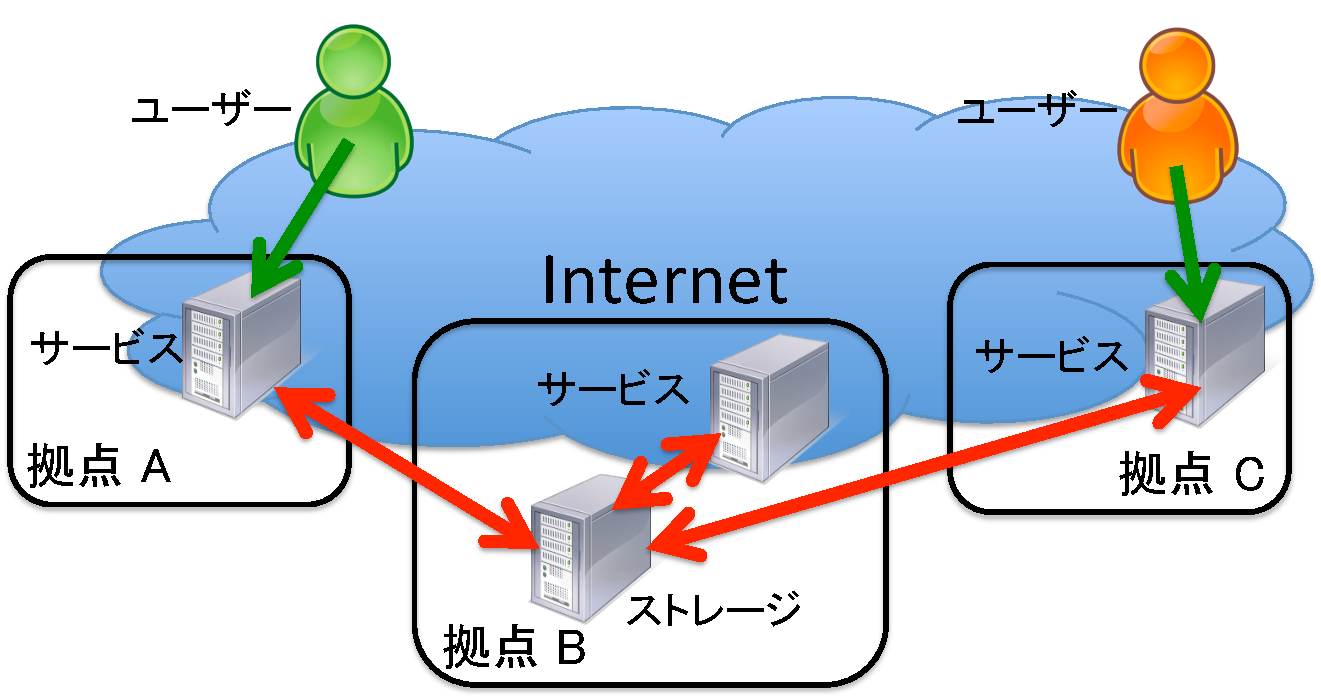
\includegraphics[scale=0.50]{./img/serviceanduser}
%         \caption{複数の拠点から提供されるサービス}
%         \label{img:mlservice}
%     \end{center}
% \end{figure}


\section{本研究が着目する課題}
\label{introduction:issue}

Swiftコンパイラが抱える他の問題との優先度や使用しているフレームワークとのつなぎ込みに関する問題が解決したとしても、SwiftコンパイラのBootstrapを行うかどうかという判断を下すにはより根源的な課題がある。
それは、現在Swiftを記述しているC++言語がSwiftと比較しても高い表現力を持っているために、~\ref{explain-bootstrap:instance}節で見る幾つかの事例とは異なり、Bootstrapを行うことで得られるメリットや、そもそも現行のコンパイラで使用されている手法を維持したままBootstrapを行うことが可能であるか否かが自明でないというものである。

また、現在のSwiftはC++との相互運用性を持っていないため、コンパイラ中の一部分をSwiftで記述したものに置き換えることは難しく、逆に実際に使用されているコンパイラ中のモジュール化が可能なほど大きなパーツをSwiftへ移植するとなると、その間の言語への機能追加などの改変は現行のものと移植中のものの両者に適用するか、移植中のもののみに追加して移植が完了するまでその適用を先送りしなくてはならなくなってしまう。


\section{本研究の目的}
\label{introduction:purpose}

本研究では、SwiftコンパイラがBootstrapすることによって得られるメリットと被るデメリットを定量的に示し、Bootstrapを行うべきか否かを判断する上で有用な情報を収集することを目的とする。
そのためのアプローチとして、Swiftコンパイラの基幹的機能である構文解析器をSwiftによって実装し、その実行時間とソースコードの行数を現行のSwiftコンパイラの構文解析器と比較する。
また、この独自の構文解析器は現行のSwiftコンパイラと基本的な設計手法において同じものを採用するだけで、完全に独立させたものとして実装する。

この方法により、現在のSwiftコンパイラの開発状況などの影響を一切受けずにBootstrapのための評価が可能となり、またその評価がBootstrapの可能性に対して有意義な知見を与えることを提示する。


\section{本論文の構成}

本論文の構成は次の通りである。

第2章では本研究の考察対象であるコンパイラのBootstrapについてSwift以外の言語の事例からそのメリットについてまとめ、Bootstrapにおける課題について整理する。
第3章では本研究が着目するプログラミング言語Swiftの特徴とそのコンパイラ実装の基幹部分における特徴について説明する。
第4章では現行のSwiftコンパイラとの比較対象となるSwiftで記述したSwiftコンパイラ「TreeSwift」の構成について述べ、現行のコンパイラとその基本的な設計手法などに大きな差異がないことを確認する。
第5章では現行のSwiftコンパイラとTreeSwiftの構文解析器についてその実行速度とソースコードの行数を比較し、その結果について考察する。
第6章では本研究の結論と今後の展望についてまとめる。

%%% Local Variables:
%%% mode: japanese-latex
%%% TeX-master: "../thesis"
%%% End:

\chapter{コンパイラのBootstrap}
\label{explain-bootstrap}

本章では、これまでにBootstrapを行ってきた高級汎用言語の事例を紹介し、それらの例からBootstrapにおける利点と課題について整理する。

\section{Bootstrapの事例}
\label{explain-bootstrap:instance}

BootstrapはFortranやLispのような比較的古い言語からGoやF\#のような比較的新しい言語まであらゆる時代の言語で行われており、その目的は様々である。
本節では、その中から特に近年よく使用されており、先に他の言語による実装が十分な機能を持ってリリースされているにもかかわらずBootstrapを行った高級汎用言語である、Goのgo、PythonのPyPy、C\#の.Net Compiler Platformの3つの事例について紹介する。

\subsection{Go - go}

Goは2009年にGoogle社より発表された、構文の簡潔さと効率の高さ、並列処理のサポートを中心的な特徴とする静的型付コンパイラ型言語である。
発表から6年を経た2015年にリリースされたバージョン1.5でBootstrapが行われ、それまでCで記述されていたコンパイラは完全にGoへと書き換わった。

\subsubsection{Bootstrapの目的}

GoコンパイラのBootstrapの目的はCとGoの比較という形で~\cite{go-compiler-overhaul}内で以下のように述べられている。

\begin{itemize}
\item It is easier to write correct Go code than to write correct C code.
\item It is easier to debug incorrect Go code than to debug incorrect C code.
\item Work on a Go compiler necessarily requires a good understanding of Go. Implementing the compiler in C adds an unnecessary second requirement.
\item Go makes parallel execution trivial compared to C.
\item Go has better standard support than C for modularity, for automated rewriting, for unit testing, and for profiling.
\item Go is much more fun to use than C.
\end{itemize}

主にGoを用いたコンパイラの開発がCを用いた場合よりも正確かつ楽になるという点を強調していることから、GoコンパイラのBootstrapの目的は主にコンパイラ開発フローの改善にあったということができるだろう。

\subsubsection{Bootstrapの方法}

Goコンパイラにおいては、~\cite{go-compiler-overhaul}に詳細なBootstrapのプロセスが記述されている。
これによれば、Bootstrapはおおまかに以下の流れで行われた。

\begin{enumerate}
\item CからGoへのコードの自動変換器を作成する。
\item 自動変換機をCで書かれたGoコンパイラに対して使用し、新しいコンパイラとする
\item 新しいGoで書かれたコンパイラをGoにとって最適な記法へと修正する
\item プロファイラの解析結果などを用いてGoで書かれたコンパイラを最適化する
\item コンパイラのフロントエンドをGoで独自に開発されているものへと変更する
\end{enumerate}

この手法では、特にCからGoへの自動変換器を作成したことで、Cで書かれたコンパイラの開発を止めること無くGoへの変換の準備を行うことができた、という点が優れている。
ただしこの手法を取れたのは、GoがCに近い機能を多く採用していたこと、CとGoが共に他の高級汎用言語と比べて少ない構文しか持っていなかったことに依るところが大きい。

また、バージョン1.5以降のGoコンパイラにおいてはまずGoのバージョン1.4を用いてコンパイルし、その後にそのコンパイラを再度自分自身でビルドすることによって最新バージョンのコンパイラでコンパイルした最新バージョンのコンパイラを得る~\cite{go-bootstrap-plan}。
この多少複雑な形によりバージョン1.5以降でもコンパイラをCから独立させることができるが、その代わりにGoのバージョン1.4に依存し続ける点には注意しなくてはならない。

\subsubsection{Bootstrapの結果}

Bootstrapが行われた結果、Goコンパイラのコンパイル速度が低下したことがバージョン1.5のリリースノート~\cite{go-15-release}で言及されている。
これについて同リリースノートではCからGoへのコード変換がGoの性能を十分に引き出せないコードへの変換を行っているためだとしており、プロファイラの解析結果などを用いた最適化が続けられている。


\subsection{Python - PyPy}

Pythonは1991年に発表されたマルチパラダイムの動的型付けインタプリタ型言語である。
Pythonの最も有名な実装であるCPythonはC言語で書かれているが、そのCPythonと互換性があり、Bootstrapされた全く別のコンパイラが2007年にPyPyという名前でリリースされている。

このPyPyではCPythonと比べてJITコンパイル機能を備えている点が最も大きな違いとなっている。

\subsubsection{Bootstrapの目的}

PyPyがBootstrapを行った目的はそのドキュメントである~\cite{pypy-doc}内の以下の記述から、特にPythonという言語の持つ柔軟性と、それによる拡張性の高さを利用するためであると読み取れる。

\begin{quotation}
This Python implementation is written in RPython as a relatively simple interpreter, in some respects easier to understand than CPython, the C reference implementation of Python. We are using its high level and flexibility to quickly experiment with features or implementation techniques in ways that would, in a traditional approach, require pervasive changes to the source code.
\end{quotation}


\subsubsection{Bootstrapの方法}

PyPyのインタプリタは、PyPyと同時に開発されているRPythonというPythonのサブセット言語で実装されており、RPythonはRPythonで書かれたプログラムをCなどのより低レベルな言語に変換する役割を担う~\cite{rpython-doc}。

そのため、RPythonの実行時の性能はPyPy自体の性能に一切関与せず、例えばPythonで記述されているRPythonがPyPyで実行されているかCPythonで実行されているかはPyPyの性能に何ら影響を与えない。

このRPythonという変換器による仲介と、既存実装であるCPythonとの互換性がPyPyのBootstrapを可能にしている。


\subsubsection{Bootstrapの結果}

PyPyについては多くのベンチマークにおいて互換性のあるCPythonのバージョンに対してその実行速度が向上していることが示されている~\cite{speed-pypy-org}。
これはPyPyが単にBootstrapを行っただけでなく、RPythonによってPyPyインタプリタをネイティブコードにコンパイルできるよう仲介した上で、JITコンパイル機能を付加したためである。

このように、Bootstrapを行ったインタプリタを直接そのインタプリタで実行するのではなく、より高速に動作する形へ変換して実行することで、性能の低下を免れられ、それどころか独自の拡張によってそれまでの実装よりもより高い性能を得られる場合がある。
ただし、この手法を取った場合はPyPyにおけるCのような他の低級言語への依存が残ってしまい、その可搬性に制限が生じてしまう可能性があるという点には注意する必要がある。


\subsection{C\# - .Net Compiler Platform}

C\#は2000年にMicrosoft社より.Net Frameworkを利用するアプリケーションの開発用に発表された、マルチパラダイムの静的型付けコンパイラ型言語である。
2014年に同社はC++で記述されていたコンパイラのBootstrapを行い、Visual Basic .NET と合わせてコンパイラ中の各モジュールをAPIによって外部から利用できるようにした.NET Compiler Platformをプレビュー版としてリリースした。
その後2015年にはVisual Studio 2015における標準のC\#コンパイラとして.NET Compiler Platformを採用するようになっている。

\subsubsection{Bootstrapの目的}

.NET Compiler Platformはコンパイラの構文解析や参照解決、フロー解析などの各ステップを独立したAPIとして提供している~\cite{roslyn-doc}。
これにより、例えばVisual StudioなどのIDEはこれらのAPIを使用することで、いちからC\#のパーサを構築すること無くシンタックスハイライトや定義箇所の参照機能を提供できる。
そうしたライブラリ的機能をスムーズに利用できるようにするためには、.NET Compiler Platform自体がそれを利用するVisual Studioの拡張などと同様の言語で提供されている必要があった。

その結果、.NET Compiler PlatformはC\#コンパイラをC\#、Visual Basic .NETをVisual Basic .NETで記述するBootstrapの形式で開発することとなっている。

\subsubsection{Bootstrapの方法}

.NET Compiler PlatformはVisual Studio 2013以前に使用されていたVisual C\#とは独立して開発され、Visual Studio 2013に採用されていたC\# 5の次期バージョンであるC\# 6の実装となっていた。
そのため、.NET Compiler Platformの開発においてVisual C\#に対する大きな変更などは行われておらず、全ての新機能を.NET Compiler Platformのみに対して適用するだけで事足りている。

また、.NET Compiler Platformの最新版はVisual Studioの最新版とともにバイナリ形式で配布されることが前提となっており、公開されているソースコードからビルドを行う場合でも配布されているコンパイラを使用する。
そのため、配布されているVisual Studioが実行可能なプラットフォーム以外で.NET Compiler Platformを使用するためにはそれを実行可能な環境でクロスコンパイルするか.NET Compiler Platform以外のC\#コンパイラを用いてコンパイルする以外に方法がないが、その明確な手立ては示されていない~\cite{roslyn-cross-platform}。

\subsubsection{Bootstrapの結果}

Microsoft社ではBootstrapを行うにあたってその性能に対して非常に注力しており、結果としてBootstrap後も想定していた充分によい性能が発揮できていると~\cite{roslyn-performance}内で述べている。

\section{Bootstrapの利点}
\label{explain-bootstrap:merit}

\section{Bootstrapの課題}
\label{explain-bootstrap:issue}

\subsection{卵が先か鶏が先か問題}

\subsection{新機能の追加}

\subsection{依存フレームワークの対応}

\subsection{性能の低下}

%%% Local Variables:
%%% mode: japanese-latex
%%% TeX-master: "../bthesis"
%%% End:

\chapter{プログラミング言語Swift}
\label{rw}

\section{Swiftの目的}
\label{rw:pointtopoint}


\section{Swiftコンパイラの構成}
\label{background:korekara}

\section{Swiftコンパイラの基幹的機能}

\section{Swiftコンパイラの課題}

%%% Local Variables:
%%% mode: japanese-latex
%%% TeX-master: "../yummy_bthesis"
%%% End:

\chapter{TreeSwiftの設計と実装}
\label{treeswift}

本章では、~\ref{explain-swift}章で述べた現行のSwiftコンパイラの特徴から比較対象となるSwiftで記述したSwiftコンパイラTreeSwiftの構文解析器が満たすべき特徴を整理し、それがどのように実装されているかについて述べる。

\section{構文解析器が満たすべき特徴}
\label{treeswift:requirements}

Bootstrapを行う上でBootstrap後のコンパイラが満たすべき要件は、基本的にはその言語の仕様を満たしていることと、以前よりも性能が改善されていること以外にはない。
しかし、本研究では現行のSwiftコンパイラと比較し考察することが目的であるため、評価を行うために必要な同一の特徴を保持している必要がある。
以下では、その特徴について述べる。

\subsubsection{LL(k)方式の採用}

現行のコンパイラの構文解析器と同等の解析力とエラー検出力、拡張性を保持していることを保証するため、TreeSwiftでもLL(k)方式の構文解析器をSwiftで書き下すことにより実装を行う。

\subsubsection{エラー文の分離}

エラー文の書き方によるソースコードの分量の変化を防ぐため、エラー文自体は構文解析器自体と別のファイルに定義し、それを参照する形を取る。

\subsubsection{構文解析以外の部分の分離}

現行のコンパイラとの比較時に比較箇所が行う処理の差が出ないようにするため、型の推論や検査など構文解析以外の部分を構文解析器から分離する。


\section{実装の概要}

本節では~\ref{treeswift:requirements}節で示した特徴を満たしながら、TreeSwiftがどのように実装されているかを説明する。


\subsection{構文解析機能}

ソースコードの構文を解析し、ASTにまとめ上げる処理は字句解析と構文解析の2つのステップに分けることができる。

\subsubsection{字句解析}

TreeSwiftでは図%~\ref{img:treeswift-lex} TODO
のように、入力となるソースコードの文字を1字ずつ読みながら分類し、リテラルや識別子、予約語といった文字数の定まっていないトークンについてはそれぞれに専用の状態遷移機械によって生成する。

\subsubsection{構文解析}

解析に使用する構文はApple社の提供するSwiftの公式ドキュメントにある構文をベースとするが、本資料は多くの誤りを含んでおりかつLL(k)形式では解析不可能な左再帰を含んでいるため、それらを取り除いた独自の構文定義を使用している。

また、TreeSwiftでは~\ref{explain-swift:structure:parser}節で述べていたような現行のSwiftコンパイラが判断できていない構文についても、独自の構文定義の追加によって構文的に分類・区別している。
そのため、TreeSwiftでは全ての構文について構文解析が完了した時点で曖昧性が排除されている。


\subsection{参照解決機能}

変数や型などの参照を解決する機能の実現には、スコープを管理し、解決しなければならない。
また、参照解決を行うタイミングもその言語仕様に合わせた選択が必要となる。

\subsubsection{参照解決のタイミング}

TreeSwiftでは~\ref{explain-swift:structure:parser}節で述べた現行のSwiftコンパイラの参照解決とは異なり、構文解析中には一切の参照解決を行わない。
そのため、構文解析が完了して参照解決を行う際にはすでにすべての参照解決が可能であることが保証されており、参照解決を構文解析の本体から分離することが可能となっている。

\subsubsection{スコープ解決}

TreeSwiftにおけるスコープの解決は構文解析時にASTとは別に構築されるスコープツリーを用いて行う。

スコープツリーでは分岐やループ、複合型の宣言などに伴って切り替わるスコープの入れ子構造を木として表現し、木の各ノードがそのスコープ内で宣言された変数や関数、型などをメンバとして保持する。
また、木の各ノードは後の参照解決のためにスコープ内で参照された変数や関数、型などの情報も保持する。

この構造により、参照解決時には木の各ノードを走査し、各参照情報についてその直近の親ノードから順に参照の対象がメンバとして含まれているかを遡って確認していけば、参照解決を行うことができるようになる。


\subsection{構文解析器のその他の機能}

\subsubsection{エラーの処理}

TreeSwiftの実行中に発見されたソースコードのエラーは構文解析ステップを通して同じ1つのインスタンスによって処理される。
構文解析器からはエラーを発見した時点でエラー文の参照と解析対象に関する情報をそのインスタンスに渡す。
そのエラーが致命的なものであった場合や、エラーを管理するインスタンスに設定された既定値よりも多くのエラーが報告されていた場合は、その時点でSwiftのエラーハンドリング機能を用いて解析中の構文の関数を抜け、エラー表示などの処理を行う。


\subsubsection{ライブラリの扱い}

TreeSwiftでは独自のバイナリ形式を使用している現行のSwiftコンパイラとは異なり、標準ライブラリを含むライブラリ内に定義されている変数や関数、型などの情報を保持するモジュール情報ファイルをテキストファイルで管理している。
それらのライブラリはimport文によって要求された時か、標準ライブラリの場合はプログラマがインプットした全てのソースコードの解析前に一度だけ解析され、一般的なソースコードと同様のASTを形成する。

ただし、ライブラリのモジュール情報ファイルでは複数のファイルにまたがったグローバル変数などの定義は存在しないため、構文解析中に即座に参照解決を行う。


\subsection{構文解析以外の実装}


\section{解析可能な構文の検証}

本節では、TreeSwiftを用いて実際に構文の解析を行った結果によってTreeSwiftが十分な構文解析機能を持っていることを示す。

\subsection{検証するプログラム}

\subsection{検証の結果}

\subsection{検証のまとめ}

%%% Local Variables:
%%% mode: japanese-latex
%%% TeX-master: "../bthesis"
%%% End:

\chapter{評価}
\label{conclusion}

本章では、本論文のまとめと今後の展望を示す。

\section{評価概要}

本研究では、インターネット上の複数の拠点に同一のLayer 2ネットワークを拡張することができる一対多型のLayer 2ネットワーク
拡張技術であるLEONの設計と実装をした。現在のインターネットには、宛先と直接通信した場合より、他の拠点を経由して宛先と通信
した場合の方が、通信をする際の遅延が小さくなる場合がある。LEONはトンネル終端点間の遅延を計測し、その計測結果をもとに遅延が最も
遅延が小さくなる経路を計算する。これにより、LEONを利用することにより、イーサネットフレームを遅延の最も小さい経路で転送できるようになった。
その結果、本研究で行った実験から、LEONを利用して拡張されたLayer 2ネットワーク上で通信を行った場合、従来手法と比べ、
サービスを構成するコンポーネントのパフォーマンスが改善され、サービスのパフォーマンスも改善されるということがわかった。
しかし、LEONでは全てのトンネル終端点が他のトンネル終端点の状態管理や遅延計測などを行う必要があるため、
トンネル終端点が増加することによりトンネル終端点の負荷が高くなるため様々な悪影響が生じる。
本研究で行った実験から、トンネル終端点の増加が与える影響の1つとして、中継を行なっているトンネル終端点での障害発生から、そのトンネル終端点を経由していた通信が再び可能になるまで
かかる時間の増加があるということがわかった。そのため、LEONは多くの拠点にLayer 2ネットワークを拡張するには適していない
ということもわかった。

\section{構文解析における性能差}

本研究で提案したLayer 2ネットワーク拡張技術であるLEONは、中継を行なっているトンネル終端点で障害が発生してから、
再びそのトンネル終端点を中継して行われていた通信が行えるようになるまで、最大で120秒かかる。そのため、最大120秒間、通信が行えない
間に、送信されたイーサネットフレームがパケットロスされてしまう可能性やサーバーから切断されてしまうなどといった
問題の原因となることが想定される。また、図~\ref{img:tenbou1}で示すように、ファイアーウォールの設定や拠点間のネットワーク
障害などにより、直接通信することはできないが、他のトンネル終端点からは到達することができる場合が考えられる。LEONは
このよう場合、直接通信することができないトンネル終端点は障害発生と判断し、トンネル終端点リストから消去してしまう。
そのため、Layer 2ネットワークが分断してしまうという問題がある。これらの問題を解決するためには、より優れた障害検知
の手法が必要である。

\begin{figure}
	\begin{center}
		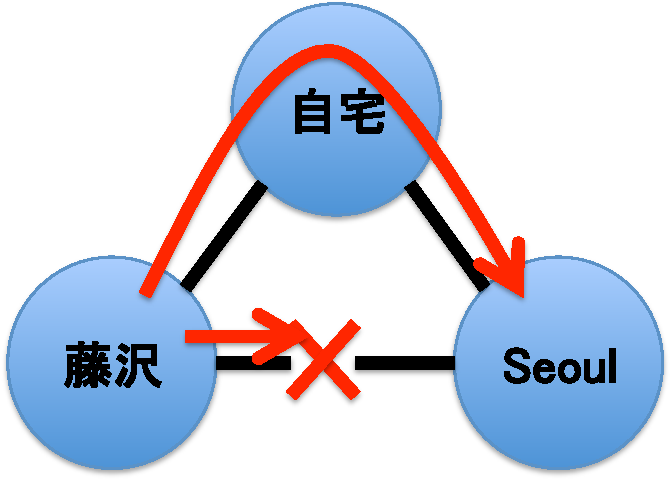
\includegraphics[scale=0.60]{./img/tenbou1}
		\caption{直接通信をすることができない状況}
		\label{img:tenbou1}
	\end{center}
\end{figure}

また、本研究で提案した手法は、トンネル終端点間の遅延を計測し、その計測結果をもとに経路の計算を行った。しかし、インターネット
には遅延は小さいが帯域幅は細いトンネル終端点や、遅延は大きいが帯域幅は太いトンネル終端点が存在する可能性がある。WIDE Cloudの
ように拡張されたLayer 2ネットワーク上で様々なアプリケーションが動作するような環境では、遅延よりも帯域幅を優先したほうがパフォーマンス
が高くなるアプリケーションも動作している可能性がある。そのため、Layer 2ネットワーク拡張技術はトンネル終端点間の遅延だけでなく、Layer 2ネットワーク上
で動作するアプリケーションやトンネル終端点間の帯域幅も考慮する必要がある。

\section{ソースコードの比較}

\section{考察}

%%% Local Variables:
%%% mode: japanese-latex
%%% TeX-master: "../yummy_bthesis"
%%% End:

\chapter{結論}
\label{conclusion}

本章では、本研究のまとめと今後の展望を示す。

\section{本研究のまとめ}

本研究では、現行のC++で記述されたSwiftコンパイラをBootstrapすることによって利益を得られるかどうかを判断することを目的として、実際にSwiftで記述したSwiftコンパイラを実装し、コンパイラの基幹機能である構文解析器について現行のコンパイラとの比較を行った。
実装したコンパイラの構文解析器はソースコードの行数から柔軟性と拡張性の変化を判断し、実行速度と実行時のメモリ使用量から性能の変化を判断するために、現行のコンパイラと同様の手法で設計した上で、同等の機能を有していることを示した。

ソースコードの行数、実行速度、実行時のメモリ使用量を比較した結果から、SwiftでSwiftコンパイラを記述することによりコンパイラの柔軟性と拡張性を向上できるが、性能については下がる可能性があり、他の利点や課題を考慮にいれると現時点におけるSwiftコンパイラについてはBootstrapによって十分な利益が得られない可能性が高いことを示した。


\section{今後の展望}

\subsection{構文解析器以外の比較}

\subsection{継続的な比較}

%%% Local Variables:
%%% mode: japanese-latex
%%% TeX-master: "../thesis"
%%% End:

\chapter*{謝辞}
\addcontentsline{toc}{chapter}{謝辞}
\label{thanks}

本論文の作成にあたり、ご指導いただきました慶應義塾大学環境情報学部教授村井純博士、同学部教授中村修博士、同学部准教授 Rodney D. Van Meter III 博士に感謝致します。

研究について日頃からご指導頂きました松谷健史氏、空閑洋平氏に感謝致します。
研究室に所属したばかりの頃から本研究に至るまで、特定の分野にこだわらない広い視点から絶えず多くのご指導をいただきました。
本研究を卒業論文としてまとめることができたのも両氏のおかげです。重ねて感謝申し上げます。

研究室を通じた生活の中で多くの示唆を与えてくださった髙橋俊成氏、Arch研究グループの皆様に感謝します。

また、徳田・村井・楠本・中村・高汐・バンミーター・植原・三次・中澤・武田合同研究プロジェクトの皆様に感謝致します。

%%% Local Variables:
%%% mode: japanese-latex
%%% TeX-master: "../yummy_bthesis"
%%% End:


\renewcommand{\thechapter}{\Alph{chapter}}
\setcounter{chapter}{0}
\vspace{-5mm}


\bibliographystyle{unsrt}\pagestyle{plain}
\bibliography{./bib/cites,./bib/bootstrapping_evidence,./bib/appendix}\pagestyle{plain}
\thispagestyle{empty}%bibtex


\end{document}

%%% Local Variables:
%%% mode: japanese-latex
%%% TeX-master: t
%%% End:
